% 2009 年天津卷文科第 11 题：AA_1 与 BB_1 相交于 O，AB∥A_1B_1 且 AB=½A_1B_1。
% 来源 PDF：普通高考/2009/2009天津文.pdf，SHA256 5d3e0110cc9145311eed3af1cf0f691ee327cbcba3a0d245e88d635fc136203f
% 原页：第 1 页（A3 三栏）第 2 栏中部，印刷页 563。
% 重绘依据：AB 与 A_1B_1 为两条平行线段，按原图呈「X」形交叉（A 连 A_1、B 连 B_1），
%   O 为交点；AB 较短、A_1B_1 较长，长度比 1:2。
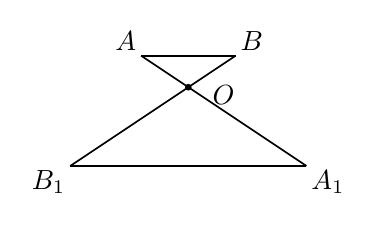
\begin{tikzpicture}[scale=1.0, semithick, every node/.style={inner sep=1.5pt}]
  \coordinate (A)  at (0.9,1.4);
  \coordinate (B)  at (2.1,1.4);
  \coordinate (B1) at (0,0);
  \coordinate (A1) at (3.0,0);
  \coordinate (O)  at (1.5,1.0);
  \draw (A) -- (B);
  \draw (A1) -- (B1);
  \draw (A) -- (A1);
  \draw (B) -- (B1);
  \fill (O) circle (1.2pt);
  \node[anchor=south east] at (A) {$A$};
  \node[anchor=south west] at (B) {$B$};
  \node[anchor=north east] at (B1) {$B_1$};
  \node[anchor=north west] at (A1) {$A_1$};
  \node[anchor=west] at ([xshift=7pt,yshift=-3pt]O) {$O$};
\end{tikzpicture}
